\documentclass{standalone}
\usepackage{tikz}
\usepackage{xcolor}
\usepackage{amsmath}
\usepackage{amssymb}
\usetikzlibrary{shapes,arrows,positioning,fit,calc,decorations.pathreplacing}

\definecolor{functioncolor}{RGB}{220,220,220}
\definecolor{loopcolor}{RGB}{255,240,245}
\definecolor{datacolor}{RGB}{240,248,255}
\definecolor{resultcolor}{RGB}{240,255,240}

\begin{document}

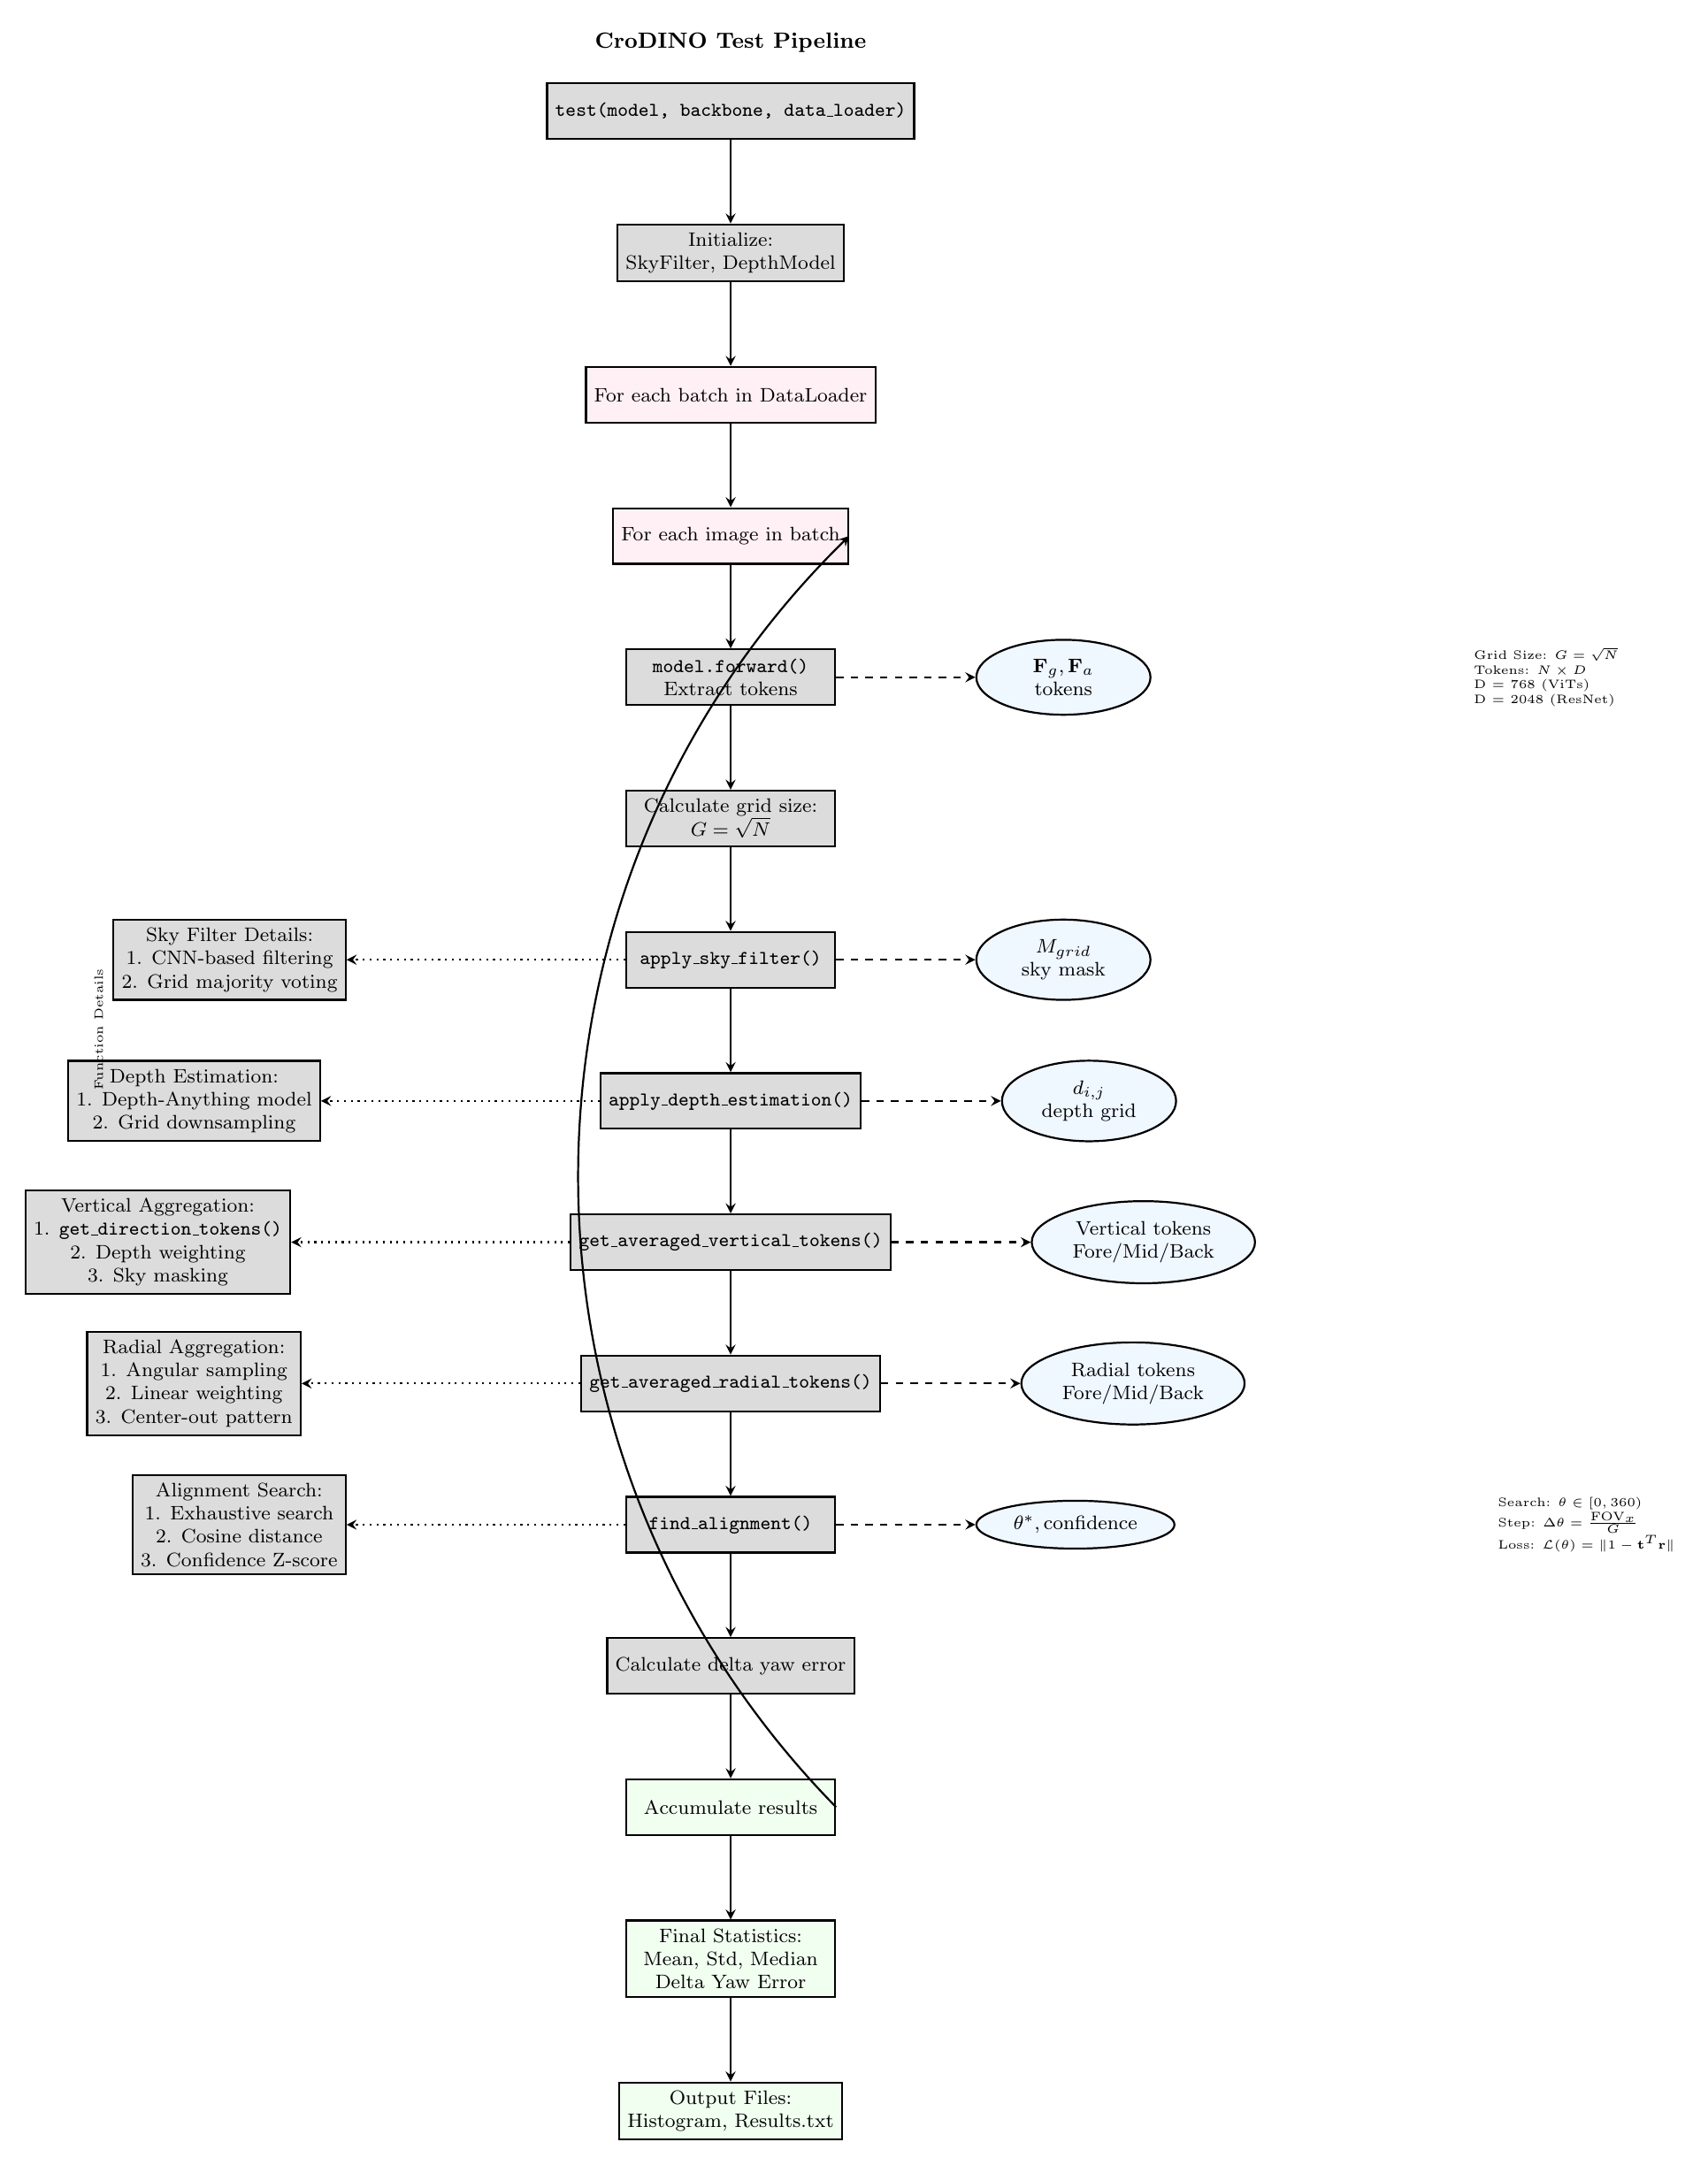
\begin{tikzpicture}[
    node distance=1.2cm,
    auto,
    thick,
    func/.style={rectangle, draw, font=\footnotesize, align=center, minimum width=3cm, minimum height=0.8cm, fill=functioncolor},
    loop/.style={rectangle, draw, font=\footnotesize, align=center, minimum width=3cm, minimum height=0.8cm, fill=loopcolor},
    data/.style={ellipse, draw, font=\footnotesize, align=center, minimum width=2.5cm, minimum height=0.6cm, fill=datacolor},
    result/.style={rectangle, draw, font=\footnotesize, align=center, minimum width=3cm, minimum height=0.8cm, fill=resultcolor},
    arrow/.style={->, >=stealth, thick}
]

% Main Function Entry
\node[func] (main) {\texttt{test(model, backbone, data\_loader)}};

% Initialization
\node[func, below=of main] (init) {Initialize:\\SkyFilter, DepthModel};

% Main Processing Loop
\node[loop, below=of init] (batch_loop) {For each batch in DataLoader};
\node[loop, below=of batch_loop] (image_loop) {For each image in batch};

% Image Processing Pipeline
\node[func, below=of image_loop] (forward) {\texttt{model.forward()}\\Extract tokens};
\node[data, right=2cm of forward] (tokens_data) {$\mathbf{F}_g, \mathbf{F}_a$\\tokens};

\node[func, below=of forward] (calc_grid) {Calculate grid size:\\$G = \sqrt{N}$};

\node[func, below=of calc_grid] (sky_func) {\texttt{apply\_sky\_filter()}};
\node[data, right=2cm of sky_func] (sky_data) {$M_{grid}$\\sky mask};

\node[func, below=of sky_func] (depth_func) {\texttt{apply\_depth\_estimation()}};
\node[data, right=2cm of depth_func] (depth_data) {$d_{i,j}$\\depth grid};

\node[func, below=of depth_func] (vert_agg) {\texttt{get\_averaged\_vertical\_tokens()}};
\node[data, right=2cm of vert_agg] (vert_data) {Vertical tokens\\Fore/Mid/Back};

\node[func, below=of vert_agg] (rad_agg) {\texttt{get\_averaged\_radial\_tokens()}};
\node[data, right=2cm of rad_agg] (rad_data) {Radial tokens\\Fore/Mid/Back};

\node[func, below=of rad_agg] (alignment) {\texttt{find\_alignment()}};
\node[data, right=2cm of alignment] (align_data) {$\theta^*, \text{confidence}$};

\node[func, below=of alignment] (error_calc) {Calculate delta yaw error};
\node[result, below=of error_calc] (accumulate) {Accumulate results};

% Detailed Function Breakdown (Left Side)
\node[func, left=4cm of sky_func] (sky_detail) {Sky Filter Details:\\1. CNN-based filtering\\2. Grid majority voting};

\node[func, left=4cm of depth_func] (depth_detail) {Depth Estimation:\\1. Depth-Anything model\\2. Grid downsampling};

\node[func, left=4cm of vert_agg] (vert_detail) {Vertical Aggregation:\\1. \texttt{get\_direction\_tokens()}\\2. Depth weighting\\3. Sky masking};

\node[func, left=4cm of rad_agg] (rad_detail) {Radial Aggregation:\\1. Angular sampling\\2. Linear weighting\\3. Center-out pattern};

\node[func, left=4cm of alignment] (align_detail) {Alignment Search:\\1. Exhaustive search\\2. Cosine distance\\3. Confidence Z-score};

% Final Results
\node[result, below=of accumulate] (final_stats) {Final Statistics:\\Mean, Std, Median\\Delta Yaw Error};

\node[result, below=of final_stats] (output_files) {Output Files:\\Histogram, Results.txt};

% Arrows - Main Flow
\draw[arrow] (main) -- (init);
\draw[arrow] (init) -- (batch_loop);
\draw[arrow] (batch_loop) -- (image_loop);
\draw[arrow] (image_loop) -- (forward);
\draw[arrow] (forward) -- (calc_grid);
\draw[arrow] (calc_grid) -- (sky_func);
\draw[arrow] (sky_func) -- (depth_func);
\draw[arrow] (depth_func) -- (vert_agg);
\draw[arrow] (vert_agg) -- (rad_agg);
\draw[arrow] (rad_agg) -- (alignment);
\draw[arrow] (alignment) -- (error_calc);
\draw[arrow] (error_calc) -- (accumulate);

% Data Flow Arrows
\draw[arrow, dashed] (forward) -- (tokens_data);
\draw[arrow, dashed] (sky_func) -- (sky_data);
\draw[arrow, dashed] (depth_func) -- (depth_data);
\draw[arrow, dashed] (vert_agg) -- (vert_data);
\draw[arrow, dashed] (rad_agg) -- (rad_data);
\draw[arrow, dashed] (alignment) -- (align_data);

% Detail Connections
\draw[arrow, dotted] (sky_func) -- (sky_detail);
\draw[arrow, dotted] (depth_func) -- (depth_detail);
\draw[arrow, dotted] (vert_agg) -- (vert_detail);
\draw[arrow, dotted] (rad_agg) -- (rad_detail);
\draw[arrow, dotted] (alignment) -- (align_detail);

% Loop back arrow
\draw[arrow, bend left=45] (accumulate.east) to (image_loop.east);

% Final output
\draw[arrow] (accumulate) -- (final_stats);
\draw[arrow] (final_stats) -- (output_files);

% Section Labels
\node[above=0.3cm of main, font=\small\bfseries] {CroDINO Test Pipeline};
\node[left=0.2cm of sky_detail, font=\tiny, rotate=90] {Function Details};

% Mathematical annotations
\node[right=4.5cm of tokens_data, font=\tiny, align=left] {
    Grid Size: $G = \sqrt{N}$\\
    Tokens: $N \times D$\\
    D = 768 (ViTs)\\
    D = 2048 (ResNet)
};

\node[right=4.5cm of align_data, font=\tiny, align=left] {
    Search: $\theta \in [0, 360)$\\
    Step: $\Delta\theta = \frac{\text{FOV}_x}{G}$\\
    Loss: $\mathcal{L}(\theta) = \|1 - \mathbf{t}^T\mathbf{r}\|$
};

\end{tikzpicture}

\end{document}
